
%%%%%%%%%%%%%%%%%%%%%%%%%%%%%%%%%%%%%%%%%%%%%%%%%%%%%%%%%%%%%%%%%%%%%
%% Please do not use \input{...} to include other tex files.       %%
%% Submit your LaTeX manuscript as one .tex document.              %%
% Note (ET): We will do this at the end!
%%                                                                 %%
%% All additional figures and files should be attached             %%
%% separately and not embedded in the \TeX\ document itself.       %%
% TODO: discuss this! might mean we have to generate all figures externaly
%%%%%%%%%%%%%%%%%%%%%%%%%%%%%%%%%%%%%%%%%%%%%%%%%%%%%%%%%%%%%%%%%%%%%
% some aditional \documentclass options:
% \documentclass[referee,...]{sn-jnl}% referee option is meant for double line spacing
%\documentclass[lineno,...]{sn-jnl}% to print line numbers in the margin use lineno option
\RequirePackage{tikz}
\documentclass[pdflatex,sn-basic]{template/sn-jnl}% Basic Springer Nature Reference Style/Chemistry Reference Style
%%\documentclass[sn-mathphys]{sn-jnl}% Math and Physical Sciences Reference Style
%%\documentclass[sn-aps]{sn-jnl}% American Physical Society (APS) Reference Style
%%\documentclass[sn-vancouver]{sn-jnl}% Vancouver Reference Style
%%\documentclass[sn-apa]{sn-jnl}% APA Reference Style
%%\documentclass[sn-standardnature]{sn-jnl}% Standard Nature Portfolio Reference Style
%%\documentclass[default]{sn-jnl}% Default
%%\documentclass[default,iicol]{sn-jnl}% Default with double column layout


%%%% Standard Packages
%%<additional latex packages if required can be included here>
%%%%%%%%%%%%%%%%%%%%%%%%%%%%%%%%%%%%%%%%%%%%%%%%%%%
%% definitions of variables
%%%%%%%%%%%%%%%%%%%%%%%%%%%%%%%%%%%%%%%%%%%%%%%%%
% general symbols
%%%%%%%%%%%%%%%%%%%%%%%%%%%%%%%%%%%%%%%%%%%%%%%%%
\DeclareMathOperator{\tr}{tr}
\newcommand{\bA}{\boldsymbol{A}}
\newcommand{\bI}{\boldsymbol{I}}
\newcommand{\bL}{\boldsymbol{L}}
\newcommand{\bvarepsilon}{\boldsymbol{\varepsilon}}
\newcommand{\bsigma}{\boldsymbol{\sigma}}
\newcommand{\TP}{^\text{T}}
%%%%%%%%%%%%%%%%%%%%%%%%%%%%%%%%%%%%%%%%%%%%%%%%%
% homogenization vars
%%%%%%%%%%%%%%%%%%%%%%%%%%%%%%%%%%%%%%%%%%%%%%%%%
\newcommand{\eMod}{E}  % youngs modulus
\newcommand{\eModEff}{\eMod_{\text{eff}}}  % mocroscopic youngs modulus
\newcommand{\poission}{\nu}  % poissionsratio
\newcommand{\poissionZero}{\poission^{(0)}}  % poissionsratio
\newcommand{\poissionEff}{\poission_{\text{eff}}}  % poissionsratio effective
\newcommand{\fc}{f_{\text{c}}}  % compressive strength
\newcommand{\fcInf}{{\fc}_\infty}  % compressive strength
\newcommand{\ft}{f_{\text{t}}}  % tensile strength
\newcommand{\ftInf}{{\ft}_\infty}  % compressive strength
\newcommand{\fcEff}{{\fc}_{,\text{eff}}}  % compressive strength
\newcommand{\body}{\Omega}  % body
\newcommand{\phaseIndex}{r}  % index letter for different phases
\newcommand{\matrixIndex}{\text{m}}  % index letter for different phases
\newcommand{\inclIndex}{\text{i}}  % index letter for different phases
\newcommand{\bodyPhase}{\body^{(\phaseIndex)}}
\newcommand{\volFrac}{c}
\newcommand{\volFracPhase}{\volFrac^{(\phaseIndex)}}
\newcommand{\volFracMatrix}{\volFrac^{(\matrixIndex)}}
\newcommand{\volFracIncl}{\volFrac^{(\inclIndex)}}
\newcommand{\volFracZero}{\volFrac^{(0)}}
\newcommand{\radius}{R}
\newcommand{\radiusPhase}{\radius^{(\phaseIndex)}}
\newcommand{\bulkMod}{K}
\newcommand{\bulkModPhase}{\bulkMod^{(\phaseIndex)}}
\newcommand{\bulkModMatrix}{\bulkMod^{(\matrixIndex)}}
\newcommand{\bulkModIncl}{\bulkMod^{(\inclIndex)}}
\newcommand{\bulkModZero}{\bulkMod^{(0)}}
\newcommand{\bulkModEff}{\bulkMod_{\text{eff}}}
\newcommand{\shearMod}{G}
\newcommand{\shearModPhase}{\shearMod^{(\phaseIndex)}}
\newcommand{\shearModMatrix}{\shearMod^{(\matrixIndex)}}
\newcommand{\shearModIncl}{\shearMod^{(\inclIndex)}}
\newcommand{\shearModZero}{\shearMod^{(0)}}
\newcommand{\shearModEff}{\shearMod_{\text{eff}}}
\newcommand{\matStiff}{\bL}
\newcommand{\matStiffZero}{\matStiff^{(0)}}
\newcommand{\matStiffPhase}{\matStiff^{(\phaseIndex)}}
\newcommand{\matStiffEff}{\matStiff_{\text{eff}}}
\newcommand{\orthProjV}{\bI_{\text{V}}}
\newcommand{\orthProjD}{\bI_{\text{D}}}
\newcommand{\strain}{\bvarepsilon}
\newcommand{\strainPhase}{\strain^{(\phaseIndex)}}
\newcommand{\strainZero}{\strain^{(0)}}
\newcommand{\stress}{\bsigma}
\newcommand{\stressZero}{\stress^{(0)}}
\newcommand{\stressMatrix}{\stress^{(\matrixIndex)}}
\newcommand{\stressD}{\stress_{\text{D}}}
\newcommand{\stressTest}{\stress^{\text{test}}}
\newcommand{\concentration}{\bA}
\newcommand{\concentrationPhase}{\concentration^{(\phaseIndex)}}
\newcommand{\concentrationZero}{\concentration^{(0)}}
\newcommand{\dilConcentration}{\concentration_{\text{dil}}}
\newcommand{\dilConcentrationPhase}{\dilConcentration^{(\phaseIndex)}}
\newcommand{\dilConcentrationIncl}{\dilConcentration^{(\inclIndex)}}
\newcommand{\dilConcentrationVPhase}{A^{(\phaseIndex)}_{\text{dil,V}}}
\newcommand{\dilConcentrationDPhase}{A^{(\phaseIndex)}_{\text{dil,D}}}
\newcommand{\dilConcentrationVIncl}{A^{(\inclIndex)}_{\text{dil,V}}}
\newcommand{\dilConcentrationDIncl}{A^{(\inclIndex)}_{\text{dil,D}}}
\newcommand{\auxAlphaZero}{\alpha^{(0)}}
\newcommand{\auxBetaZero}{\beta^{(0)}}
\newcommand{\Jtwo}{J_2}
\newcommand{\JtwoTest}{\Jtwo^{\text{test}}}
\newcommand{\JtwoZero}{\Jtwo^{(0)}}
\newcommand{\JtwoMatrix}{\Jtwo^{(\matrixIndex)}}
\newcommand{\force}{f} 
\newcommand{\forceTest}{\force^{\text{test}}} 
\newcommand{\thermCond}{\chi}
\newcommand{\thermCondZero}{\thermCond^{(0)}}
\newcommand{\thermCondPhase}{\thermCond^{(\phaseIndex)}}
\newcommand{\thermCondMatrix}{\thermCond^{(\matrixIndex)}}
\newcommand{\thermCondIncl}{\thermCond^{(\inclIndex)}}
\newcommand{\thermCondHom}{\thermCond_{\text{eff}}}
\newcommand{\concentrationThermCondPhase}{A_{\chi}^{(\phaseIndex)}}
\newcommand{\concentrationThermCondIncl}{A_{\chi}^{(\inclIndex)}}
\newcommand{\Ivol}{\bI_{\text{V}}}
\newcommand{\Idev}{\bI_{\text{D}}}
%%%%%%%%%%%%%%%%%%%%%%%%%%%%%%%%%%%%%%%%%%%%%%%%%
% fem model vars
%%%%%%%%%%%%%%%%%%%%%%%%%%%%%%%%%%%%%%%%%%%%%%%%%
\newcommand{\currentn}{n+1}
\newcommand{\lastn}{n}
\newcommand{\DOH}{\alpha} % degree of hydration
\newcommand{\DOHLast}{\DOH^{\lastn}} % degree of hydration of last timestep
\newcommand{\DOHCurrent}{\DOH^{\currentn}} % degree of hydration of last timestep
\newcommand{\DOHmax}{\alpha_{\text{max}}} % degree of hydration
\newcommand{\DOHt}{\alpha_{\text{t}}} % degree of hydration
\newcommand{\DOHZero}{\alpha_{0}} % degree of hydration
\newcommand{\heat}{Q} % cummulative heat release
\newcommand{\heatInf}{Q_{\infty}} % total cummulative heat release
\newcommand{\zeit}{t} % time
\newcommand{\temp}{T} % time
\newcommand{\tempCurrent}{\temp^{\currentn}} % time n+1
\newcommand{\tempLast}{\temp^{\lastn}} % time n
\newcommand{\tempRef}{\temp_{\text{ref}}}
\newcommand{\dTdt}{\frac{\partial \temp}{\partial \zeit}}  % time derivative of temperature
\newcommand{\dQdt}{\frac{\partial \heat}{\partial \zeit}}  % time derivative of heat
\newcommand{\heatCapSpecific}{C} % specific heat capacity
\newcommand{\density}{\rho} % density
\newcommand{\thermCondEff}{\lambda} % effective thermal conductivity %%% \thermCond
\newcommand{\dDOHdt}{\frac{\partial \DOH}{\partial \zeit}}  % time derivative of DoH
\newcommand{\affinity}{A} % temperature \affinityTempscaled affinity
\newcommand{\affinityTemp}{\tilde{\affinity}} % temperature \affinityTempscaled affinity
\newcommand{\affinityScale}{a} % scale factor for affinity
\newcommand{\hydParBone}{B_1}
\newcommand{\hydParBtwo}{B_2}
\newcommand{\hydParEta}{\eta}
\newcommand{\function}{f}
\newcommand{\strengthX}{X}
\newcommand{\strengthXInf}{\strengthX_\infty}
\newcommand{\strengthExp}{a}
\newcommand{\strengthXExp}{\strengthExp_\strengthX}
\newcommand{\strengthCExp}{\strengthExp_{\fc}}
\newcommand{\strengthTExp}{\strengthExp_{\ft}}
\newcommand{\stiffExp}{\strengthExp_{\eMod}}
\newcommand{\eModInf}{\eMod_\infty}  % youngs modulus
\newcommand{\activE}{E_{\text{a}}}
\newcommand{\gasConst}{R}
\newcommand{\wc}{r_{\text{wc}}}
%%%%%%%%%%%%%%%%%%%%%%%%%%%%%%%%%%%%%%%%%%%%%%%%%
% beam design vars
%%%%%%%%%%%%%%%%%%%%%%%%%%%%%%%%%%%%%%%%%%%%%%%%%
\newcommand{\beamLength}{l}
\newcommand{\beamDistrLoad}{q}
\newcommand{\beamPointLoad}{F}
\newcommand{\beamMaxMoment}{M_{\text{max}}}
\newcommand{\beamMaxShearForce}{F_{\tau,\text{max}}}
\newcommand{\beamHeight}{h}
\newcommand{\beamHeightEff}{\beamHeight_{\text{eff}}}
\newcommand{\beamCover}{c}
\newcommand{\beamSteelDiameter}{d_{\text{st}}}
\newcommand{\beamConcreteSF}{\gamma_{\text{c}}}
\newcommand{\beamSteelSF}{\gamma_{\text{s}}}
\newcommand{\beamTimeSF}{\alpha_{\text{cc}}}
\newcommand{\beamfcd}{f_{\text{cd}}}
\newcommand{\beamfsd}{f_{\text{ywd}}}
\newcommand{\beamfs}{f_{\text{yk}}}





  % tex commands not variable
\newcommand{\workflowGraph}{paper_workflow_graph.gv.pdf}
\newcommand{\snakemakeGraph}{snakemake_optimization_graph.pdf}
   % tex commands created by script
%%%%%%%%%%%%%%%%%%%%%%%%%%%%%%%%%%%%%%%%%%%%%%%%%%%%%%%%%%%
%% Shotcuts used by TUM DDMM -------------------------
%%%%%%%%%%%%%%%%%%%%%%%%%%%%%%%%%%%%%%%%%%%%%%%%%%%%%%%%%%%

\newcommand{\refeq}[1]{Equation \eqref{#1}}
\newcommand{\boxeq}[1]{%
  \[\fbox{%
      \addtolength{\linewidth}{-2\fboxsep}%
      \addtolength{\linewidth}{-2\fboxrule}%
      \begin{minipage}{\linewidth}%
      \begin{equation}#1\end{equation}%
      \end{minipage}%
    }\]%
}
%%%%%%%%%%%%%%%%%%%%%%%%%%%%%%%%%%%%%%%%%%%%%%%%%%%%%%%
\newcommand{\ee}{\end{equation}}
\newcommand{\be}{\begin{equation}}
\newcommand{\ec}{\end{center}}
\newcommand{\bc}{\begin{center}}
\newcommand{\eea}{\end{eqnarray}}
\newcommand{\bea}{\begin{eqnarray}}
\newcommand{\bd}{\begin{description}}
\newcommand{\ed}{\end{description}}
\newcommand{\bi}{\begin{itemize}}
\newcommand{\ei}{\end{itemize}}
\newcommand{\pa}{\partial}

\newcommand{\bx}{\bs{x}}
\newcommand{\bxi}{\bx^{(i)}}
\newcommand{\bxn}{\bx^{(n)}}

\newcommand{\by}{\bs{y}}
\newcommand{\byn}{\by^{(n)}}
\newcommand{\bs}{\boldsymbol}

%\newcommand{\br}{\bs{r}} 
\newcommand{\brn}{\bs{r}^{(n)}} 

\newcommand{\bz}{\bs{z}}
\newcommand{\pt}{p^{trans}}

\newcommand{\bxx}{\bs{X}}
\newcommand{\bxb}{\bar{\bs{X}}}
\newcommand{\byy}{\bs{Y}}

\newcommand{\bt}{\bs{\theta}}
\newcommand{\btt}{\bs{\Theta}}


\newcommand{\bp}{\bs{\phi}}

\newcommand{\beps}{\bs{\epsilon}}
\newcommand{\qe}{q_{\epsilon}(\bs{\epsilon})}

\newcommand{\bax}{\bs{A}_x}
\newcommand{\bbx}{\bs{b}_x}
\newcommand{\bvx}{\bs{V}_x}
\newcommand{\bcx}{\bs{C}_x}
\newcommand{\bdx}{\bs{D}_x}
\newcommand{\E}{\mathbb{E}}



\newcommand{\psk}[1]{{\color{red} PSK: #1}}
\newcommand{\atul}[1]{{\color{green} AA: #1}}



% preamble stuff
\usepackage{subfigure}
\usepackage{amsmath,bm}
\usepackage{amssymb}
\usepackage{mdframed}
\usepackage{tikz}
\usetikzlibrary{graphs,graphs.standard}


\newcommand{\figures}{../figures/} % scale factor for affinity
%%%%

%%%%%=============================================================================%%%%
%%%%  Remarks: This template is provided to aid authors with the preparation
%%%%  of original research articles intended for submission to journals published 
%%%%  by Springer Nature. The guidance has been prepared in partnership with 
%%%%  production teams to conform to Springer Nature technical requirements. 
%%%%  Editorial and presentation requirements differ among journal portfolios and 
%%%%  research disciplines. You may find sections in this template are irrelevant 
%%%%  to your work and are empowered to omit any such section if allowed by the 
%%%%  journal you intend to submit to. The submission guidelines and policies 
%%%%  of the journal take precedence. A detailed User Manual is available in the 
%%%%  template package for technical guidance.
%%%%%=============================================================================%%%%

\jyear{2022}%


\raggedbottom
%%\unnumbered% uncomment this for unnumbered level heads

\begin{document}
\title[From concrete mixture to structural design - a holistic optimization procedure]{From concrete mixture to structural design - a holistic optimization procedure}

%%=============================================================%%
%% Prefix	-> \pfx{Dr}
%% GivenName	-> \fnm{Joergen W.}
%% Particle	-> \spfx{van der} -> surname prefix
%% FamilyName	-> \sur{Ploeg}
%% Suffix	-> \sfx{IV}
%% NatureName	-> \tanm{Poet Laureate} -> Title after name
%% Degrees	-> \dgr{MSc, PhD}
%% \author*[1,2]{\pfx{Dr} \fnm{Joergen W.} \spfx{van der} \sur{Ploeg} \sfx{IV} \tanm{Poet Laureate} 
%%                 \dgr{MSc, PhD}}\email{iauthor@gmail.com}
%%=============================================================%%
% TODO: discuss order of authors, do we need to include more?


\author*[1]{\fnm{Atul} \sur{Agrawal}}\email{atul.agrawal@tum.de}
\equalcont{These authors contributed equally to this work.}

\author[2]{\fnm{Erik} \sur{Tamsen}}\email{erik.tamsen@bam.de}
\equalcont{These authors contributed equally to this work.}

\author[1]{\fnm{Faidon-Stelios} \sur{Koutsourelakis}}\email{p.s.koutsourelakis@tum.de}

\author[2]{\fnm{Jörg F.} \sur{Unger}}\email{joerg.unger@bam.de}

\affil*[1]{\orgdiv{Data-driven Materials Modeling}, \orgname{Technische Universität München}, \orgaddress{\street{Boltzmannstraße 15}, \city{Garching}, \postcode{85748}, \country{Germany}}}

\affil[2]{\orgdiv{Modeling and Simulation}, \orgname{Bundesanstalt für Materialforschung und -prüfung}, \orgaddress{\street{Unter den Eichen 87}, \city{Berlin}, \postcode{12205}, \country{Germany}}}


%%==================================%%
%% sample for unstructured abstract %%
%%==================================%%
\abstract{Amazing introduction to this topic, talking about problems with local optimization on mix and structre.
We are ...
By applying .... stochastic methods, the quality of the data can be estimated.
Automated workflow to simplify addition of additional data points and general reproducibility.}

\keywords{performance oriented design, stochastic optimization, precast concrete, mix design}

%%\pacs[JEL Classification]{D8, H51}

%%\pacs[MSC Classification]{35A01, 65L10, 65L12, 65L20, 65L70}

\maketitle


\section{Introduction}\label{sec:introduction}
Precast concrete elements play a critical role in achieving efficient, low cost and sustainable structures.
The controlled production environment allows for higher quality products and enables the mass production of elements.
In the standard design approach, engineers or architects select a structure, estimate the loads, choose mechanical properties, and design the element accordingly. 
If the results are not satisfactory, the required mechanical properties are iteratively adjusted, aiming to improve the design.
This approach is fine, when the choice of mixtures is limited and the expected concrete properties are well known.
There are various published methods to automate this process and optimize the beam design at this level.
Computer aided beam design optimization dates back at least 50 year, e.g. \cite{Haung1967}.
Generally the objective is reducing costs, with the design variables being the beam geometry, the amount and location of the reinforcement and sometimes the compressive strength of the concrete \cite{Chakrabarty_1992, Coello_1997, Pierott_2021, Shobeiri_2023} .
Most publications focus on analytical functions based on norms and well known rules of thumb.
In recent years the use of alternative binders in the concrete mix design has increased, mainly to reduce the environmental impact and cost of concrete but also to improve and modify specific properties.
This is a challenge as the concrete mix is no longer a constant and is itself subjected to optimization.
Known heuristics might no longer apply to the new materials and old design approaches might fail to produce optimal results.
In addition it is not favorable to choose from a predetermined set of possible mixes, as this would either lead to an exaggerated number of required experiments or a limiting subset of the possible design space.
There exist literature studying the optimization of specific concrete properties on the concrete mix \cite{Lisienkova_2021, Kondapally_2022}.
\begin{figure}[b]%
	\centering
	\includegraphics[width=1.0\textwidth]{../figures/\designStandard}
	\caption{Classical design approach, where the required material properties are defined before the mix is defined.}\label{fig:standard_design}
\end{figure}
The objective in that literature is normally to either improve some mechanical property like durability within constraints, or to minimize e.g. the amount of concrete while keeping other properties above a threshold.
When designing elements subjected to various requirements, both on the material and structural level, including workability of the fresh concrete, durability of the structure, maximum acceptable temperature, minimal cost and global warming potential, the optimal solution is not apparent and will change depending on each individual project.
The conventional method of design does not allow for an concurrent optimization of structural measures and concrete mix composition, as the structural  design and the concrete mix design are inversely coupled, c.f. Figure \ref{fig:standard_design}.
The lack of coordination between the designer and the concrete manufacturer can therefore lead to suboptimal solutions, as neither party possesses all the relevant information.
A first step to address these limitations is the incorporation of compressive strength during a optimization in the beam design phase.
Higher compressive strength usually correlates with lager amount of cement and therefore higher cost as well as global warming potential.
This approach has shown promising results in achieving improved structural efficiency while considering environmental impact \cite{dos_Santos_2023}.
To be able to find a part specific optimum, individual data of the manufacturer and specific mix options must be integrated.
Therefore, there is still a need for a comprehensive optimization procedure that can seamlessly integrate concrete mixture optimization and structural simulations, ensuring structurally sound and buildable elements with minimized environmental impact for part specific data.
\\
\begin{figure}[b]%
	\centering
	\includegraphics[width=1.0\textwidth]{../figures/\designProposed}
	\caption{Presented design approach that allows for a holistic optimization.}\label{fig:proposed_workflow}
\end{figure}
%%%%%%%%%%%%%%%%%%%%
In this paper, we present a holistic optimization procedure that combines concrete mixture optimization with the structural response of precast concrete elements, using structural simulations as constraints to ensure structural integrity, limit the maximum temperature and ensure an adequate time of demolding.
This inverts the classical design pipeline.
As a first step the concrete mix is defined.
Based on the output, the beam design is created, c.f. Figure \ref{fig:proposed_workflow}.
The chosen example of this optimization procedure is to reduce the GWP of precast concrete elements. 
By integrating the concrete mixture optimization and structural design processes, engineers can tailor the concrete properties to meet specific requirements of the customer and manufacturer.
This approach opens up possibilities for performance prediction and optimization for new mixture that fall outside the standard range of well-known concrete.
To the best of our knowledge there are no published works that combine the material and structural level in one flexible optimization framework.
In addition to changing the order of the design steps, the proposed framework allows to directly integrate experimental data and propagate the identified uncertainties.
This allows a straight forward integration of new data and and quantification of uncertainties regarding the predictions.
The proposed framework consists of three main parts.
First, an automated and reproducible parameter identification method to calibrate the models.
Second, a gradient-based optimization method for non-differentiable functions, including constraints.
Third, a flexible workflow combining the models and functions required for the respective problem. 
For this publication a well known example of a simply supported, reinforced, rectangular beam  has been chosen.
The design problem was originally published in \cite{everard1966reinforced}.
It has been used to showcase different optimization schemes, e.g. \cite{Chakrabarty_1992}, \cite{Coello_1997}, \cite{Pierott_2021}.
The experimental data used in the parameter identification step is mainly sourced from \cite{gruyaert2011}.
The objective is to reduce the overall global warming potential of the part.
This objective is a particularly meaningful as the cement industry, a major contributor to GWP, accounts for approximately 8\% of the total anthropogenic GWP. 
Reducing the environmental impact of cement production becomes crucial in the pursuit of sustainable construction practices.
In addition, the reduction of cement is also correlated to the reduction of cost, as cement is generally the most expensive component of the concrete mix \cite{Paya_Zaforteza_2009}.
There are three direct ways to reduce the amount of cement.
First, replace the cement with a substitute with a lower carbon footprint.
This can change mechanical properties, but does not necessarily mean a reduction in strength.
Second, increase the amount of aggregates.
This also changes effective properties and needs to be balanced with the workability and the limits due to the applications.
Third, decrease the overall volume of concrete.
In addition, when analyzing the whole life-cycle of concrete, both cost and GWP can be reduced by increasing the durability and therefore extending the lifetime of the object.
To showcase the methods capability, two design variables have been chosen, the height of the beam and the ratio of ordinary Portland cement (OPC) to its replacement binder ground granulated blast furnace slack, a by-product of iron industry.\\
%
The value of this manuscript lies in two main contributions. 
Firstly, it presents the possibility to automatically compute relevant Key Performance Indicators (KPIs) at the structural level, based on input values that incorporate parameters relevant to the concrete mix design, inverting the classical design pipeline.
This allows for a comprehensive evaluation of both structural performance and environmental impact. 
Secondly, the paper details the numerical methods employed to conduct a robust optimization process without derivatives, taking into account uncertainties based on raw experimental data.
\\
% this might change and needs to be adapted
The paper starts  with the theoretical background of the parameter identification method in Section \ref{sec:calibration}.
It is followed by the optimization method in Section \ref{sec:optimization} and some numerical experiments showcasing the method in \ref{sec:numericalexperiments}.
Section \ref{sec:data} gives details on the example problem and an overview of the available experimental data.
The following Section \ref{sec:models} gives an overview of the material models and applied assumption. 
In Section \ref{sec:results} all parts, the experimental data, the calibration method, the numerical models and the optimization framework are combined to demonstrate the effectiveness and practicality of the proposed approach.
The publication finishes with a conclusion and outlook in Section \ref{sec:conclusion}.

\section{Experimental data}\label{sec:data}
Description and overview of experimental data used.
\ET{This section still needs to be written.
	I think all relevant infos should be found in the PhD thesis that provided the data.
	It should just give an overview of what data was available and was used.}
\subsection{Young's modulus \texorpdfstring{$\eMod$}{E} based on \texorpdfstring{$fc$}{fc}}
The dataset does not encompass information about Young's modulus. 
Given its significance for  the FEM simulation, we resort to a phenomenological approximation derived from \cite{ACI363}. 
This approximation relies on the compressive strength $\fc$ and the density $\density$ to estimate the Young's modulus
\begin{align}
	\eMod = 3320 \sqrt{\fc} + 6895 \left( \dfrac{\density}{2320}\right)^{1.5}.
\end{align}
We opt to approximate $\eMod$ prior to the identification and learning phases. 
Often, both Young's modulus and compressive strength data are available. 
Our intention is to demonstrate the feasibility of considering these parameters separately as a proof of concept.

\section{Models}\label{sec:models}
\subsection{Notes on micromechanic based concrete homogenization}

\cite{mor_1973_asi} original paper of mt method\\
\cite{str_2011_mbeo} mori tanaka homogenization of thermal conductivity\\
\cite{nev_2018_mcam} description of fc value\\
\cite{nee_2012_ammf} description of E homogenization\\
\cite{pic_2011_uqso} similar ansatz, multiscale homogenization including wc focus\\
\cite{her_1993_nlib} paper with correct coating formulation




This manuscript gives an overview of the implementation used within my concrete simulation.
The goal is to compute effective concrete parameters based on information of the micro constituents.
In particular the cement paste and aggregates are considered.
It is possible to consider air pores as well as the influence of the interfacial transition zone (IFZ) as a coat surrounding aggregates with reduced stiffness. 
First the estimation of the effective Young's modulus $\eModEff$ and Poisson's ratio $\poissionEff$ is given.
It is based on the classical analytical Mori-Tanaka homogenization formulation \cite{mor_1973_asi} for spherical inclusions in a matrix.
This is extended to the case of a coated inclusions, following \cite{her_1993_nlib}.
In general the implementation of the stiffness homogenization is following the formulations presented in \cite{nee_2012_ammf}, however the appendix includes some errors, where the original paper \cite{her_1993_nlib} should be consulted.
Subsequently the estimation of the effective compressive strength $\fcEff$ is given, following the ideas of \cite{nev_2018_mcam}.

\subsection{Stiffness homogenization as presented in \cite{nee_2012_ammf}}
The general idea of this analytical homogenization procedure is to describe the overall stiffness of a body $\body$, based on the properties of the individual phases, i.e. the matrix and the inclusions.
Each of the $n$ phases is denoted by the index $\phaseIndex$, where $\phaseIndex = 0$ is defined as the matrix phase.
The volume fraction of each phase is defined as
\begin{align}
	\volFracPhase = \frac{\left\| \bodyPhase \right\|}{\left\| \body \right\|} \quad  \text{for}~ \phaseIndex = 0, ..., n.
\end{align}
The inclusions are assumed to be spheres, defined by their radius $\radiusPhase$.
The shells are defined by their outer radius, their thickness follows as the difference to the inner inclusions.
The elastic properties of each homogeneous and isotropic phase is given by the material stiffness matrix $\bL^{(\phaseIndex)}$, here written in terms of the bulk and shear moduli $\bulkMod$ and $\shearMod$,
\begin{align}
	\matStiffPhase= 3 \bulkModPhase \orthProjV + 2 \shearModPhase \orthProjD  \quad \text{for}~ \phaseIndex = 0, ..., n, \label{eq:Lr}
\end{align}
where $\orthProjV$ and $\orthProjD$ are the orthogonal projections of the volumetric and deviatoric components.\\
The methods assumes that the micro-heterogeneous body $\body$ is subjected to a macroscale strain $\strain$.
It is assumed that for each phase concentration factor $\concentrationPhase$ can be defined such that
\begin{align}
	\strainPhase = \concentrationPhase\strain \quad  \text{for}~ \phaseIndex = 0, ..., n, \label{eq:strainaverage}
\end{align}
which computes the average strain $\strainPhase$ based on the overall strains.
This can then be used to compute the effective stiffness matrix $\matStiffEff$ as a volumetric sum over the constituents weighted by the concentration factor 
\begin{align}
	\matStiffEff = \sum_{\phaseIndex=0}^{n} \volFracPhase \matStiffPhase\concentrationPhase \quad  \text{for}~ \phaseIndex = 0, ..., n.\label{eq:Leff}
\end{align}

The concentration factors $\concentrationPhase$,
\begin{align}
	\concentrationZero &= \left( \volFracZero\bI + \sum^{n}_{\phaseIndex=1} \volFracPhase \dilConcentrationPhase\right)^{-1}\label{eq:A0}\\
	\concentrationPhase &= \dilConcentrationPhase\concentrationZero\quad  \text{for}~ \phaseIndex = 1, ..., n,
\end{align}
are based on the dilute concentration factors $\dilConcentrationPhase$, which need to be obtained first.
The dilute concentration factors are based on the assumption that each inclusion is subjected to the average strain in the matrix $\strainZero$.
\begin{align}
	\strainPhase = \dilConcentrationPhase\strainZero \quad  \text{for}~ \phaseIndex = 1, ..., n. 
\end{align}


The dilute concentration factors neglect the interaction among phases and are only defined for the inclusion phases $\phaseIndex = 1,...,n$.
The applied formulation uses an additive volumetric-deviatoric split. where
\begin{align}
	\dilConcentrationPhase = \dilConcentrationVPhase\Ivol +  \dilConcentrationDPhase \Idev \quad  \text{for}~ \phaseIndex = 1, ..., n,
\end{align}
This chosen method extends the basic Mori-Tanaka method the coated inclusions, following \cite{her_1993_nlib}, therefore two different formulations for the dilute concentration factors are given for the uncoated and coated inclusion. 

\subsubsection{Dilute concentration factors for uncoated inclusions}
The formulations of the dilute concentration factors for an uncoated inclusion $\phaseIndex$ are
\begin{align}
	\dilConcentrationVPhase = \dfrac{\bulkModZero}{\bulkModZero + \auxAlphaZero(\bulkModPhase - \bulkModZero)}, \\
	\dilConcentrationDPhase = \dfrac{\shearModZero}{\shearModZero + \auxBetaZero(\shearModPhase - \shearModZero)}, 
\end{align}
with the auxiliary factors following from the Eshelby solution as
\begin{align}
	\auxAlphaZero = \frac{1 + \poissionZero}{3(1+ \poissionZero)} \quad\text{and}\quad 
	\auxBetaZero = \frac{2(4 - 5\poissionZero)}{15(1 - \poissionZero)}
\end{align}
where  $\poissionZero$ refers to the Poission's ratio of the matrix phase.
\subsubsection{Effective stiffness}
Now that the formulation for the dilute concentration factor for inclusions are defined the effective bulk and shear modului can be computed based on a sum over the phases
\begin{align}
\bulkModEff = \dfrac{\volFracZero\bulkModZero + \sum^{n}_{\phaseIndex=1} \volFracPhase \bulkModPhase \dilConcentrationVPhase}{\volFracZero + \sum^{n}_{\phaseIndex=1} \volFracPhase \dilConcentrationVPhase},\label{eq:keff} \\
\shearModEff = \dfrac{\volFracZero\shearModZero + \sum^{n}_{\phaseIndex=1} \volFracPhase \shearModPhase \dilConcentrationDPhase}{\volFracZero + \sum^{n}_{\phaseIndex=1} \volFracPhase \dilConcentrationDPhase}.\label{eq:geff}
\end{align}
\subsection{Strength homogenization as presented in \cite{nev_2018_mcam}}
Based on the ideas of the previous section, a formulation is used to homogenize the effective strength of the composite.
The strength estimation is based on two main assumptions.
First assumptions, the Mori-Tanaka method is used to estimate the average stress within the matrix material, which is the indicator of overall failure.
Based on the concept of \eqref{eq:strainaverage}, with the formulations \eqref{eq:Lr},\eqref{eq:Leff} and \eqref{eq:A0}, the average matrix stress is defined as 
\begin{align}
	\stressZero = \matStiffZero\concentrationZero {\matStiffEff}^{-1}\stress. \label{eq:matrixstress}
\end{align}
Second assumption, the von Mises failure criterion is used to estimate the uniaxial compressive strength
\begin{align}
	\sqrt{3 \Jtwo} - {\fc} = 0. \label{eq:vonMises}
\end{align}
The second deviatoric stress invariant is defined as
\begin{align}
	\Jtwo = \frac{1}{2} \stressD:\stressD,\quad\text{with}\quad
	\stressD = \stress - \frac{1}{3}\tr(\stress)\bI.
\end{align}
The goal is to find a uniaxial macroscopic stress $\stress = \begin{bmatrix} -\fcEff & 0 & 0 &0&0&0 \end{bmatrix}\TP$ which exactly fulfills the von Mises failure criterion \eqref{eq:vonMises} for the average stress within the matrix $\stressZero$.
The procedure here is taken from the code provided in the link in \cite{nee_2012_ammf}.

First we compute the second deviatoric stress invariant $\JtwoTest$ for a uniaxial test stress $\stressTest = \begin{bmatrix} \forceTest & 0 & 0 &0&0&0 \end{bmatrix}\TP$. Then the matrix stress $\stressZero$ is computed based on the test stress following \eqref{eq:matrixstress}. This is used to compute the second deviatoric stress invariant $\JtwoZero$ for the average matrix stress.
Now the effective compressive strength is estimated as
\begin{align}
	\fcEff = \frac{\JtwoTest}{\JtwoZero} \forceTest.
\end{align}


\subsection{Thermal conductivity homogenization as presented in \cite{str_2011_mbeo}}
Homogenization the thermal conductivity is also based on the Mori-Tanaka method.
The formulations are similar as for the stiffness homogenization, i.e. \eqref{eq:keff} and \eqref{eq:geff}.
Here only the implemented formulation is given, no further background.
The expressions are taken from \cite{str_2011_mbeo}, Section 2.2.
The thermal conductivity $\thermCondHom$ is given as
\begin{align}
	\thermCondHom = \dfrac{\volFracZero\thermCond + \sum^{n}_{\phaseIndex=1} \volFracPhase \thermCondPhase \concentrationThermCondPhase}{\volFracZero + \sum^{n}_{\phaseIndex=1} \volFracPhase \concentrationThermCondPhase}\quad\text{and}\quad
	\concentrationThermCondPhase = \frac{3\thermCondZero}{2\thermCondZero+\thermCondPhase}.
\end{align}

\subsection{Finite Element Concrete Model}
The notable feature of the concrete model is the evolution of the mechanical properties over time.
When concrete is mixed its consistency is close to liquid.
Due to a chemical reaction of the binder with water, called hydration, crystals develop that give concrete its strength and stiffness.
The reaction is both exothermal and temperature dependent.
Therefore, the primary model computes the temperature field $\temp$ \eqref{eq:heat1} and the degree of hydration $\DOH$ \eqref{eq:doh}.
The temperature model depends on three material properties, the effective thermal conductivity $\thermCondEff$, the specific heat capacity $C$ and the heat release $\dQdt$.
The $\dQdt$ in turn is governed by the hydration model, characterized by six parameters:
$\hydParBone, \hydParBtwo, \hydParEta, \tempRef, \activE$ and $\DOHmax$.
The first three $\hydParBone, \hydParBtwo$ and $\hydParEta$ are phenomenological, numerical parameters characterizing the shape of the function of the heat release.
$\tempRef$ does not need to be identified.
It is the reference temperature for which the first three parameters are calibrated.
$\activE$ is the activation energy, defining how the model will react to temperature changes, relative the the reference. 
$\DOHmax$ is the maximum degree of hydration that can be reached.
Following \cite{Mills1966fico}, the maximum degree of hydration is estimated, based on the water to binder ratio $\wc$, as $\DOHmax = \frac{1.031\,\wc}{0.194 + \wc}$.
As the degree of hydration if difficult to quantify experimentally, the heat release is used as a proxy.
By assuming the DOH is the fraction of the currently released heat with respect to its theoretical potential $\heatInf$, the current degree of hydration is estimated as $\DOH(\zeit) = \frac{\heat(\zeit)}{\heatInf}$.
As the potential heat release is also difficult to measure, as it takes a long time to fully hydrate and will only do so under perfect conditions, we obtain this value along side the other using the parameter identification method.
Figure \ref{fig:heatrelease} shows the influence of the three numerical parameter and the potential heat release on the heat release rate as well as the cumulative heat release.
\begin{figure}[h]%
	\centering
	\includegraphics[width=1.0\textwidth]{../figures/\heatReleasePlot}
	\caption{Influence of the hydration parameters on the heat release rate and the cumulative heat release.}\label{fig:heatrelease}
\end{figure}
For a detailed model description see in Appendix \ref{appendix:fem}.
In addition to influencing the reaction speed, the computed temperature is used to verify that the maximum temperature during hydration does not exceed a limit of $\tempLimit = \inputtemperaturelimit$\textdegree C.
Above this temperature, certain crystals start to revert back to a different state, expanding in volume and leading to cracks in the concrete.
This is implemented as a constraint for the optimization problem \eqref{eq:concstraintT}.
Based on the degree of hydration, the Young's modulus $\eMod$ of a linear-elastic material model
is approximated \eqref{eq:EwrtDOH}.
Further, a compressive strength in terms of the degree of hydration is computed \eqref{eq:fcwrtDOH}, which is utilized to determine a failure criterion based on the computed local stresses \eqref{eq:constraintStress}.
For a detailed description of the parameters evolution with respect to the degree of hydration see in Appendix \ref{appendix:fem_evolution}.
Figure \ref{fig:parameterEvolution} shows the influence of the different parameters.
In addition to the presented formulations in \cite{car_2016_mamt} which depend a theoretical value of parameters for fully hydrated concrete at $\DOH = 1$, this work reformulates the equations, to depend on the 28 day values $\eModTwentyEight$ and $\fcTwentyEight$ as well as the corresponding $\DOHTwentyEight$ which is obtained via a simulation.
\begin{figure}[h]%
	\centering
	\includegraphics[width=1.0\textwidth]{../figures/\evolutionPlot}
	\caption{Influence of parameters $\DOHt, \stiffExp$ and $\strengthCExp$ on evolution the Young's modulus and the compressive strength with respect to the degree of hydration $\DOH$. }\label{fig:parameterEvolution}
\end{figure}
\subsection{Approximate concrete tensile strength based on compressive strenght}
To reduce the number of required experiments, the tensile strength of concrete is approximated using the formulations given in DIN EN 1992-1-1.
They are based on the compressive strength 
\begin{align}
\ft = 
\begin{cases}
0.3 \fc^{\frac{2}{3}}  & \text{for $\fc \le 50$ N/mm$^2$}\\
\ft =2.12 \ln \left( 1 \left( \frac{\fc + 8}{10}\right) \right)& \text{for $\fc > 50$ N/mm$^2$}  \label{eq:tensilstrength}
\end{cases}
\end{align}
\subsection{$\DOHmax$ based on $\wc$}
...
\subsection{Beam design}
...

\section{Calibration Method}\label{sec:calibration}
Here is an empty file as example to start the calibration section.
Feel free to create as many sections as necessary :D.

\atul{30 Nov, 2022: !!Below is just initial documentation. .Please dont analyze the content yet. More will be added here.!!}
%%%%%%%%%%%%%%%%%%%%%%%%%%%%%%%%%%%%%%%%%%%%%%%%%%%%%%%
% Calibration -----------------------------------------
%%%%%%%%%%%%%%%%%%%%%%%%%%%%%%%%%%%%%%%%%%%%%%%%%%%%%%%
\subsection{Model Calibration}















%%%%%%%%%%%%%%%%%%%%%%%%%%%%%%%%%%%%%%%%%%%%%%%%%%%%%%%
% Optimization -----------------------------------------
%%%%%%%%%%%%%%%%%%%%%%%%%%%%%%%%%%%%%%%%%%%%%%%%%%%%%%%

\subsection{Optimization under uncertainty}






\subsubsection{Non-differentiable objective/constraints with design variables as argument}
%
In lot of real world scenarios, complex computer simulators are used to build a relationship between parameters of the underlying theory to the experimental observations. Many a times the physics bases simulator/forward solver denoted by $\bm{y}(\cdot)$ is non-diffrentiable. For inference/optimization tasks involving these simulators, many active research areas are trying to tackle this. \cite{cranmer2020frontier, louppe_adversarial_2019, beaumont2002approximate,marjoram2003markov}. Elaborating further, if the simulator is related to the objective of some optimization problem and design variables $\bm{x}$ of the problem are direct input to the objective, then gradient based approaches are not directly applicable. The following optimization is desired:
\begin{align}
    \bm{x}^* = \min_{\bm{x}}\mathcal{O}(\bm{y}_o(\bm{x}))
\end{align}
%
For simplifying the explanation, constraints are omitted for now. In contrast to \refeq{eq:opt_a}, the design variables $\bm{x}$ are direct/explicit input to the solver. In such a setting, we advocate the use of Variational Optimization. \cite{bird_stochastic_2018,staines_variational_2012,staines2013optimization}. 

\subsubsection{\emph{Variational optimization}}
%
 Variational optimization are general optimization techniques that can be used to form a differentiable bound on the optima of a non-differentiable function. Given the objective $\mathcal{O}(\bm{y}(\bm{x}))$ with a simulator $\bm{y}(\cdot)$ to minimize (for simplicity lets call it $f(\bm{x})$ for now), these techniques are based on the following observation:

\begin{align}
    \min _{\boldsymbol{x}} f(\boldsymbol{x}) \leq \mathbb{E}_{\boldsymbol{x} \sim q(\boldsymbol{x} \mid \theta)}[f(\boldsymbol{x})]=U(\boldsymbol{\theta})
\end{align}
 where $q(\boldsymbol{x} \mid \theta)$ is a proposal distribution with parameters $\bm{\theta}$ over input values/design variables $\bm{x}$. In plain words, the minimum of a collection of values is always less than their average. Instead of minimizing $f$ with respect to $\bm{x}$, we can minimize the upper bound $U$ with respect to $\bm{\theta}$.
 
 Under mild restrictions outlined by \cite{staines_variational_2012}, the bound $U(\boldsymbol{ \theta})$ is differential w.r.t $\bm{\theta}$, and using the log-likelihood trick its gradient can be rewritten as:

\begin{align}\label{eq:grad_estimator}
\nabla_{\boldsymbol{\theta}} U(\boldsymbol{\theta}) &=\nabla_{\boldsymbol{\theta}} \mathbb{E}_{\boldsymbol{x} \sim q(\boldsymbol{x} \mid \boldsymbol{\theta})}[f(\boldsymbol{x})] \nonumber \\
&=\nabla_{\boldsymbol{\theta}} \int q(\boldsymbol{x} \mid \boldsymbol{\theta}) f(\boldsymbol{x}) d \boldsymbol{x} 
\nonumber\\
&=\int \nabla_{\boldsymbol{\theta}} q(\boldsymbol{x} \mid \boldsymbol{\theta}) f(\boldsymbol{x}) d \boldsymbol{x} 
\nonumber \\
&=\int q(\boldsymbol{x} \mid \boldsymbol{\theta}) \nabla_\theta \log q(\boldsymbol{x} \mid \boldsymbol{\theta}) f(\boldsymbol{x}) d \boldsymbol{x} 
\nonumber \\
&=\mathbb{E}_{\boldsymbol{x} \sim q(\boldsymbol{x} \mid \boldsymbol{\theta})}\left[\nabla_{\boldsymbol{\theta}} \log q(\boldsymbol{x} \mid \boldsymbol{\theta}) f(\boldsymbol{x})\right]
\end{align}

The \refeq{eq:grad_estimator} is the score function estimator\cite{glynn1990likelihood}, which also appears in the context of reinforcement learning. In the reinforcement learning context, it is classically known as the REINFORCE estimates. \cite{williams1992simple}. 

Effectively, this just means that if the score function $\nabla_{\boldsymbol{\theta}} \log q(\boldsymbol{x} \mid \boldsymbol{\theta})$ of the proposal is known and if one can evaluate $f(\bm{x})$ for any $\bm{x}$, then one can construct approximations of \refeq{eq:grad_estimator} which can in turn be used to minimize $U(\boldsymbol{\theta})$ with stochastic gradient descent. 

For samples $x^1, \dotsc, x^S$ from $q(\boldsymbol{x} \mid \boldsymbol{\theta})$  the following Monte Carlo based unbiased estimator to the upper bound gradient can be used:

\begin{align}
    \frac{\partial U}{\partial \theta} \approx \frac{1}{S} \sum_{i=1}^{S} f\left(x_i\right) \frac{\partial}{\partial \theta} \log q\left(x_i \mid \theta\right)
\end{align}

% -- Variance reduction with Baseline -------
% build up multiple design variables and all (ARM paper)
% Max welling paper and others
It is well known that the gradient estimator suffers from high variance which can depend on number of sample, nature of the simulator/solver etc. A common solution for this problem is to use a baseline \cite{williams1992simple} which makes use of the fact that:

\begin{align}
    \mathbb{E}_{\boldsymbol{x} \sim q(\boldsymbol{x} \mid \boldsymbol{\theta})}\left[\nabla_{\boldsymbol{\theta}} \log q(\boldsymbol{x} \mid \boldsymbol{\theta}) f(\boldsymbol{x})\right] = \mathbb{E}_{\boldsymbol{x} \sim q(\boldsymbol{x} \mid \boldsymbol{\theta})}\left[\nabla_{\boldsymbol{\theta}} \log q(\boldsymbol{x} \mid \boldsymbol{\theta}) (f(\boldsymbol{x}) - B)\right]
\end{align}

for any constant $B$. The choice of the $B$ does not bias the gradient estimator, but can control the variance if chosen properly. 

For estimators using multiple samples as in the case presented above, we propose the use of baseline $B_i$ for the $i-th$ term based on the other samples $j\neq i: ~~ B_i = \frac{1}{S-1} \sum_{j\neq i}f(x_j)$ as discussed in \cite{kool_buy_2022}. Doing this, we obtain the following for the estimator:

\begin{align}
        \frac{\partial U}{\partial \theta} &\approx \frac{1}{S} \sum_{i=1}^{S}  \frac{\partial}{\partial \theta} \log q\left(x_i \mid \theta\right) \left(f(x_i)-\frac{1}{S-1} \sum_{j\neq i}f(x_j)\right)\\
        &= \frac{1}{S-1} \sum_{i=1}^{S}  \frac{\partial}{\partial \theta} \log q\left(x_i \mid \theta\right) \left(f(x_i)-\frac{1}{S} \sum_{j=1}^{S}f(x_j)\right) \label{eq:baseline_trick}
\end{align}

The form in \refeq{eq:baseline_trick} is convenient as it allows to construct a fixed baseline which is to be computed once per gradient step. Its crucial to stress on the fact that this amounts to no further computational budget as the simulators/solver would be solved for $S$ number of times and the baseline uses the same dataset. For proof of the unbiasedness of the estimator in \refeq{eq:baseline_trick}, the reader is directed to the Appendix section in \cite{kool_buy_2022}.

% Our idea
% Couple variatioonal optimization, baslines, penalty based optimization, automatic computational graphs.
% -- Adding constraints how it will look like
% add why no aug lamgrangian paper


% -- In practive implementation with computaional graph 
% add computational graph paper () and explain the graph

\section{Optimization Method}\label{sec:optimization}
Here is an empty file as example to start the optimization section.


\section{Numerical Experiments}\label{sec:numericalexperiments}
\subsection{Quadratic function}
Lets consider a simple 2D quadratic function given by:
\begin{align}
	f(\bm{x}) = \frac{1}{2D}\left( x_1^2 + x_2^2\right)
\end{align}
with $\bm{x} = (x_1,x_2)$. For the function, consider the problem:
\be
\min_{\bs{x}} f(\bs{x}), \qquad \textrm{ such that $x_1 \geq 1$ }
\ee
%
Following from Eq.\ref{eq:U_theta_constraint}, the upper bound can be given by the following for a Gaussian with the variational parameter $\theta$:
\begin{align}
	U(\bm{\theta}) = \E_{\bm{x}\sim \mathcal{N}(\bm{x}\mid \bm{\theta})}\left[ f(\bm{x}) + \max (1-x_1,0)\right]
\end{align}
with $\bm{\theta} = (\mu,\sigma)$. The gradients of the upper bound $U(\bm{\theta})$ can be approximated as discussed in Eq. \ref{eq:VO_grad_estimator} using Monte Carlo. With the learning rate $\eta=0.1$, initial noise $\sigma = 5$ and ADAM optimizer to perform the optimization, we obtain the results discussed in Figure \ref{fig:VO}. Figure \ref{fig:VO_no_cons} discusses the results when the constraints are not considered and Figure \ref{fig:VO_constraints} discusses the results with the constraints. As we can see from the figures that the noisy gradient estimates are able to drive that optimizer to the minimum. Especially in the case of Figure \ref{fig:VO_constraints}, two different starting point are studied. One which starts in a domain where the constraints are met (in red) and the next where the constraints are violated (in yellow). In both the cases, the optimizer moves towards the minimum while satisfying the constraints, thus converging close to $(x_1,x_2)= (1,0)$. Its also noteworthy to observe that the variance $\sigma^2$ reduces as we near the minimum.  

\begin{figure}[!htpb]
	\centering
	\begin{subfigure}{0.75\textwidth}
		\centering
		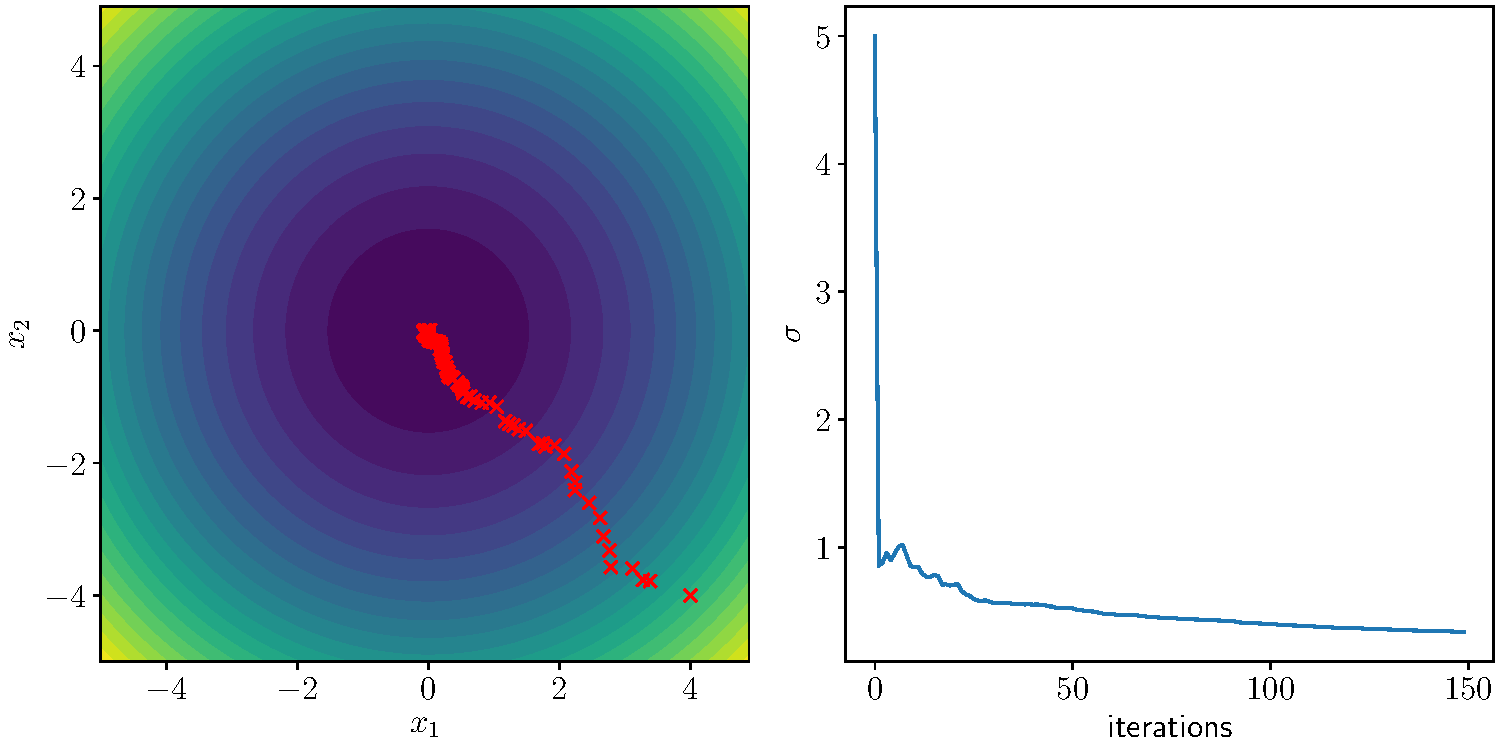
\includegraphics[width=\linewidth]{../figures/TUM/theta_evolution_VO_2023_02_21-03_34_28_PM.pdf}
		\caption{}
		\label{fig:VO_no_cons}
	\end{subfigure}
	\begin{subfigure}{0.75\textwidth}
		\centering
		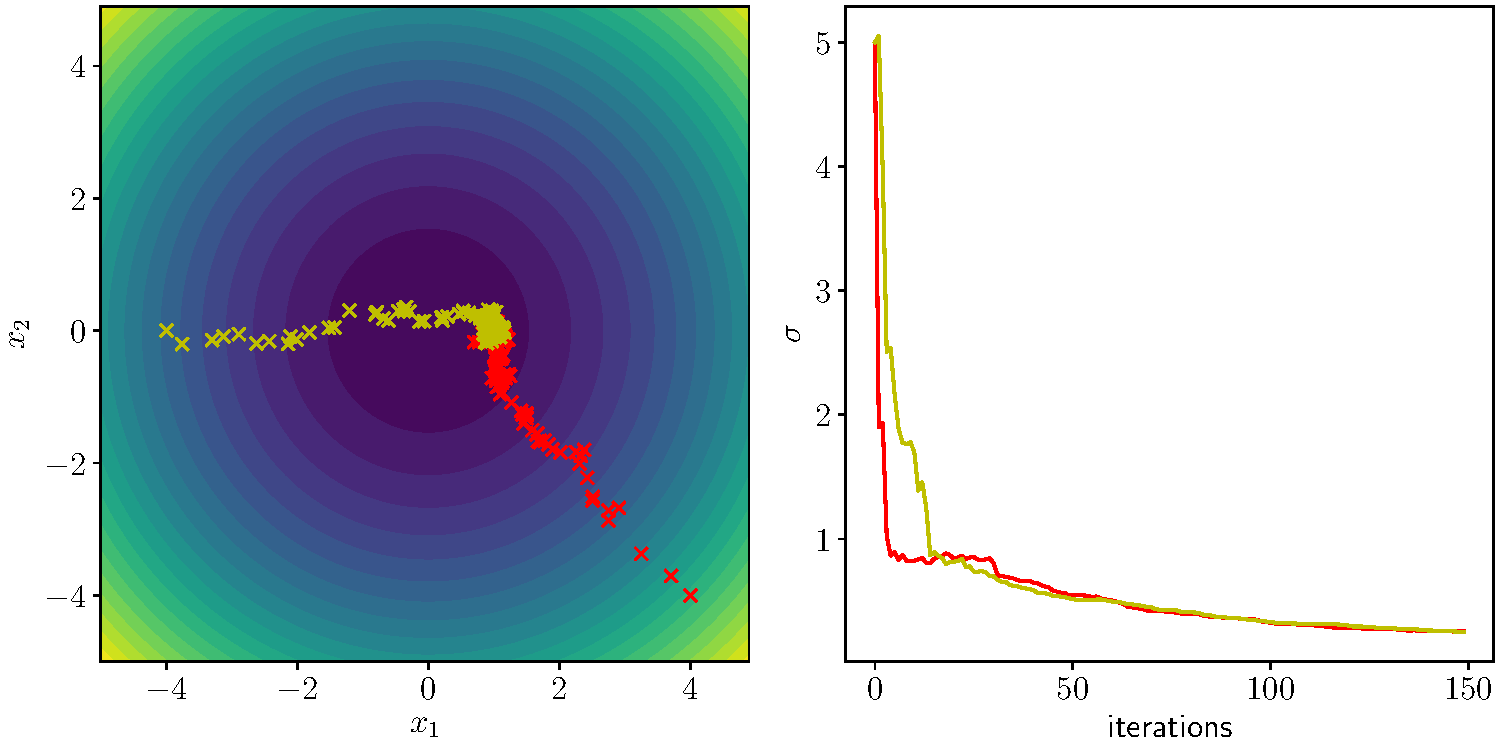
\includegraphics[width=\linewidth]{../figures/TUM/theta_evolution_VO_constraints_2023_02_24-05_12_07_PM.pdf}
		\caption{}
		\label{fig:VO_constraints}
	\end{subfigure}
	\caption{\emph{Stochastic VO for constrained and unconstrained quadratic function}: (a) This is for case when constraints are not present. The left plot shows how the Gaussian mean $\mu$ move towards the minimum of objective despite noisy gradients, the right plots the learned $\sigma$ values versus the gradient descent iterations (b) This is for a constraint on $\bm{x} (x_1 \geq 1)$. The left plot shows how the Gaussian mean $\mu$ moves towards the optimum (for two different starting values) while trying to satisfy the constraint and the right plots the learned $\sigma$ values versus the gradient descent iterations   }
	\label{fig:VO}
\end{figure}

\begin{mdframed}
	\textbf{Open research question/Novelty :} 
	\begin{enumerate}
		\item Why not use finite differences to approximate gradients?: With the constraints, the augmented objective is $C^0$, so the gradients are not even defined at that point.
		\item Then why not use Bayesian Optimization? \atul{Bayesian optimization is difficult for $(dim \geq 10)$. Also constraints are "difficult" in Bayesian optimization. The VO most probably will also struggle in high dimention. Have to check. But including constraints is not that difficult. Stelios: For the current toy problem, BO may be better (because objective has no random variable). But for the problem when the objective has implicit dependance on the design variable (through a random variable), BO makes no sense. The objective would not be known}
		\item To test in high dimention, Will it make sense to test the VO with the following?:
		\begin{align}
			f(x) = \frac{1}{200}\sum_{i=1}^{100} x_i^2 \quad \text{s.t} \quad x_i\geq1
		\end{align}
		The $\bm{x}^*$ would be a unit vector.
	\end{enumerate}
\end{mdframed}


\subsection{Performance based concrete design}

\begin{figure}[!htpb]
	\centering
	\begin{tikzpicture}
		\node (theta) at (-1,-2) {$\theta$};
		\node (x_1) at (0,0) {$x_1$};
		\node (x_2) at (0,-2) [circle, draw, dotted] {$x_2$};
		\node (b_1) at (1,1) [circle, draw] {$\bm{b}_1$}; % can add fill=black!20
		\node (b_2) at (1,0) [circle, draw] {$\bm{b}_2$};
		\node (y_1) at (3,1) [rectangle, draw] {$y_1$};
		\node (y_2) at (3,0) [rectangle, draw] {$y_2$}; 
		\node (y_3) at (3,-1) [rectangle, draw] {$y_3$}; 
		\node (y_4) at (3,-2) [rectangle, draw] {$y_4$}; 
		\node (C_1) at (5,1) [rectangle, draw] {$\mathcal{C}_1\left(y_1(\cdot)\right)$}; 
		\node (C_2) at (5,0) [rectangle, draw] {$\mathcal{C}_2\left(y_2(\cdot)\right)$}; 
		\node (C_3) at (5,-1) [rectangle, draw] {$\mathcal{C}_3\left(y_3(\cdot)\right)$}; 
		\node (O) at (5,-2) [rectangle, draw] {$\mathcal{O}\left(y_4(\cdot)\right)$}; 
		
		\graph {
			%A [as=$\mathcal{A}$, shape = none, "$P(A)$"];
			%B [as=$B$, shape=rectangle ,"$P(B)$"];
			%C [as=$C$,fill=black!20 , "$P(C|A,B)$"];
			
			(x_1) -> {(b_1),(b_2),(y_4)};
			(b_1) -> {(y_1),(y_2),(y_3)};
			(b_2) -> {(y_1),(y_2),(y_3)};
			(y_1) -> (C_1);
			(y_2) -> (C_2);
			(y_3) -> (C_3);
			(y_4) -> (O);
			(theta) -> (x_2);
			(x_2) -> {(y_1),(y_2),(y_3),(y_4)};
			
		};
	\end{tikzpicture}
	\caption{\emph{Stochastic computational graph for the constraint optimization problem for the performance based concrete design:} The circle represents \textit{stochastic nodes}, rectangle the \textit{deterministic node} and no shape is for the \textit{input nodes} (design variables). The objective and the constraints are explicitly dependant on the design variable $x_2$ and they are not differentiable w.r.t it (Hence $x_2$ in dotted). So based on our discussions above, $x_2 \sim q(x_2\mid\theta)$. Several other deterministic nodes are present between the random variables $\bm{b}_1$,$\bm{b}_2$ and the KPIs $y_1, y_2, y_3, y_4$ but they are ignored for brevity.}
	\label{fig:stochastic graph demonstrator}
\end{figure}

The interconnected graph in Figure. \ref{label} can be represented in term of probabilistic graphs as discussed in Figure. \ref{fig:stochastic graph demonstrator}

\atul{This section will involve the calibration results and then the optimization results. The concrete model discussed in section 2 IMO should be in a form accessible to computational science community, with details elaborated in Appendix. Drawing from discussions in section 2, we can discuss the results here.}

\section{Results}\label{sec:results}
Here is an empty file as example to start the results section.


\section{Conclusion and Outlook}\label{sec:results}
Here is an empty file as example to start the conclusion section.


% supplementary information, acknowledgements, declarations, etc

\backmatter

\bmhead{Supplementary information}

If your article has accompanying supplementary file/s please state so here. 

Authors reporting data from electrophoretic gels and blots should supply the full unprocessed scans for key as part of their Supplementary information. This may be requested by the editorial team/s if it is missing.

Please refer to Journal-level guidance for any specific requirements.

\bmhead{Acknowledgments}

Acknowledgments are not compulsory. Where included they should be brief. Grant or contribution numbers may be acknowledged.

Please refer to Journal-level guidance for any specific requirements.

\section*{Declarations}

Some journals require declarations to be submitted in a standardised format. Please check the Instructions for Authors of the journal to which you are submitting to see if you need to complete this section. If yes, your manuscript must contain the following sections under the heading `Declarations':

\begin{itemize}
\item Funding
\item Conflict of interest/Competing interests (check journal-specific guidelines for which heading to use)
\item Ethics approval 
\item Consent to participate
\item Consent for publication
\item Availability of data and materials
\item Code availability 
\item Authors' contributions
\end{itemize}

\noindent
If any of the sections are not relevant to your manuscript, please include the heading and write `Not applicable' for that section. 

%%===================================================%%
%% For presentation purpose, we have included        %%
%% \bigskip command. please ignore this.             %%
%%===================================================%%
\bigskip
\begin{flushleft}%
Editorial Policies for:

\bigskip\noindent
Springer journals and proceedings: \url{https://www.springer.com/gp/editorial-policies}

\bigskip\noindent
Nature Portfolio journals: \url{https://www.nature.com/nature-research/editorial-policies}

\bigskip\noindent
\textit{Scientific Reports}: \url{https://www.nature.com/srep/journal-policies/editorial-policies}

\bigskip\noindent
BMC journals: \url{https://www.biomedcentral.com/getpublished/editorial-policies}
\end{flushleft}


\begin{appendices}
\section{Mori-Tanaka Homogenization}\label{appendix:hom}
\subsection{Approximation of elastic properties}\label{ssec:mt_elastic}
The chosen method to homogenize the elastic, isotropic properties $\eMod$ and $\poission$ is the Mori-Tanaka homogenization scheme, \cite{mor_1973_asi}.
It is a well-established, analytical homogenization method.
The formulation uses bulk and shear moduli $\bulkMod$ and $\shearMod$.
They are related to $\eMod$ and $\poission$ as $\bulkMod = \frac{\eMod}{3(1-2\poission)}$ and $\shearMod = \frac{\eMod}{2(1+\poission)}$.
The used Mori-Tanaka method assumes spherical inclusions in an infinite matrix and considers the interactions of multiple inclusions.
The applied formulations follow the notation published in 
\cite{nee_2012_ammf}, where this method is applied to successfully model the effective concrete stiffness for multiple types of inclusions.
The general idea of this analytical homogenization procedure is to describe the overall stiffness of a body $\body$, based on the properties of the individual phases, i.e. the matrix and the inclusions.
Each of the $n$ phases is denoted by the index $\phaseIndex$, where $\phaseIndex = 0$ is defined as the matrix phase.
The volume fraction of each phase is defined as
\begin{align}
	\volFracPhase = \frac{\left\| \bodyPhase \right\|}{\left\| \body \right\|} \quad  \text{for}~ \phaseIndex = 0, ..., n.
\end{align}
The inclusions are assumed to be spheres, defined by their radius $\radiusPhase$.
The elastic properties of each homogeneous and isotropic phase is given by the material stiffness matrix $\bL^{(\phaseIndex)}$, here written in terms of the bulk and shear moduli $\bulkMod$ and $\shearMod$,
\begin{align}
	\matStiffPhase= 3 \bulkModPhase \orthProjV + 2 \shearModPhase \orthProjD  \quad \text{for}~ \phaseIndex = 0, ..., n, \label{eq:Lr}
\end{align}
where $\orthProjV$ and $\orthProjD$ are the orthogonal projections of the volumetric and deviatoric components.\\
The method assumes that the micro-heterogeneous body $\body$ is subjected to a macroscale strain $\strain$.
It is considered that for each phase a concentration factor $\concentrationPhase$ can be defined such that
\begin{align}
	\strainPhase = \concentrationPhase\strain \quad  \text{for}~ \phaseIndex = 0, ..., n, \label{eq:strainaverage}
\end{align}
which computes the average strain $\strainPhase$ within a phase, based on the overall strains.
This can then be used to compute the effective stiffness matrix $\matStiffEff$ as a volumetric sum over the constituents weighted by the corresponding concentration factor 
\begin{align}
	\matStiffEff = \sum_{\phaseIndex=0}^{n} \volFracPhase \matStiffPhase\concentrationPhase \quad  \text{for}~ \phaseIndex = 0, ..., n.\label{eq:Leff}
\end{align}

The concentration factors $\concentrationPhase$,
\begin{align}
	\concentrationZero &= \left( \volFracZero\bI + \sum^{n}_{\phaseIndex=1} \volFracPhase \dilConcentrationPhase\right)^{-1}\label{eq:A0}\\
	\concentrationPhase &= \dilConcentrationPhase\concentrationZero\quad  \text{for}~ \phaseIndex = 1, ..., n,
\end{align}
are based on the dilute concentration factors $\dilConcentrationPhase$, which need to be obtained first.
The dilute concentration factors are based on the assumption that each inclusion is subjected to the average strain in the matrix $\strainZero$, therefore
\begin{align}
	\strainPhase = \dilConcentrationPhase\strainZero \quad  \text{for}~ \phaseIndex = 1, ..., n. 
\end{align}
The dilute concentration factors neglect the interaction among phases and are only defined for the inclusion phases $\phaseIndex = 1,...,n$.
The applied formulation uses an additive volumetric-deviatoric split, where
\begin{align}
	\dilConcentrationPhase = \dilConcentrationVPhase\Ivol +  \dilConcentrationDPhase \Idev \quad  \text{for}~ \phaseIndex = 1, ..., n, \text{\quad with}
\end{align}
\begin{align}
	\dilConcentrationVPhase = \dfrac{\bulkModZero}{\bulkModZero + \auxAlphaZero(\bulkModPhase - \bulkModZero)}, \\
	\dilConcentrationDPhase = \dfrac{\shearModZero}{\shearModZero + \auxBetaZero(\shearModPhase - \shearModZero)}.
\end{align}
The auxiliary factors follow from the Eshelby solution as
\begin{align}
	\auxAlphaZero = \frac{1 + \poissionZero}{3(1+ \poissionZero)} \quad\text{and}\quad 
	\auxBetaZero = \frac{2(4 - 5\poissionZero)}{15(1 - \poissionZero)}
\end{align}
where  $\poissionZero$ refers to the Poission's ratio of the matrix phase.
The effective bulk and shear modului can be computed based on a sum over the phases
\begin{align}
\bulkModEff = \dfrac{\volFracZero\bulkModZero + \sum^{n}_{\phaseIndex=1} \volFracPhase \bulkModPhase \dilConcentrationVPhase}{\volFracZero + \sum^{n}_{\phaseIndex=1} \volFracPhase \dilConcentrationVPhase},\label{eq:keff} \\
\shearModEff = \dfrac{\volFracZero\shearModZero + \sum^{n}_{\phaseIndex=1} \volFracPhase \shearModPhase \dilConcentrationDPhase}{\volFracZero + \sum^{n}_{\phaseIndex=1} \volFracPhase \dilConcentrationDPhase}.\label{eq:geff}
\end{align}
Based on the concept of \eqref{eq:strainaverage}, with the formulations \eqref{eq:Lr},\eqref{eq:Leff} and \eqref{eq:A0}, the average matrix stress is defined as 
\begin{align}
\stressZero = \matStiffZero\concentrationZero {\matStiffEff}^{-1}\stress. \label{eq:matrixstress}
\end{align}
\subsubsection{Approximation of compressive strength}\label{ssec:compressivestrength}
The estimation of the concrete compressive strength $\fcEff$ follows the ideas of \cite{nev_2018_mcam}.
The procedure here is taken from the code provided in the link in \cite{nee_2012_ammf}.
The assumption is that a failure in the cement paste will cause the concrete to crack.
The approach is based on two main assumptions.
First, the Mori-Tanaka method is used to estimate the average stress within the matrix material $\stressMatrix$. 
The formulation is given in \eqref{eq:matrixstress}.
Second, the von Mises failure criterion of the average matrix stress is used to estimate the uniaxial compressive strength
\begin{align}
	{\fc} = \sqrt{3 \Jtwo},  \label{eq:vonMises}
\end{align}
with $\Jtwo(\stress) = \frac{1}{2} \stressD:\stressD$ and $\stressD = \stress - \frac{1}{3}\tr(\stress)\bI$.
It is achieved by finding a uniaxial macroscopic stress $\stress = \begin{bmatrix} -\fcEff & 0 & 0 &0&0&0 \end{bmatrix}\TP$, which exactly fulfills the von Mises failure criterion \eqref{eq:vonMises} for the average stress within the matrix $\stressMatrix$.
The procedure here is taken from the code provided in the link in \cite{nee_2012_ammf}.
First a $\JtwoTest$ is computed for a uniaxial test stress $\stressTest = \begin{bmatrix} \forceTest & 0 & 0 &0&0&0 \end{bmatrix}\TP$. 
Then the matrix stress $\stressMatrix$ is computed based on the test stress following \eqref{eq:matrixstress}. 
This is used to compute the second deviatoric stress invariant $\JtwoMatrix$ for the average matrix stress.
Finally the effective compressive strength is estimated as
\begin{align}
	\fcEff = \frac{\JtwoTest}{\JtwoMatrix} \forceTest.
\end{align}
\subsubsection{Approximation of thermal conductivity}\label{ssec:thermalconductivity}
Homogenization of the thermal conductivity is based on the Mori-Tanaka method as well.
The formulation is similar to \eqref{eq:keff} and \eqref{eq:geff}.
The expressions are taken from \cite{str_2011_mbeo}.
The thermal conductivity $\thermCondHom$ is computed as
\begin{align}
	\thermCondHom = \dfrac{\volFracMatrix\thermCondMatrix + \volFracIncl \thermCondIncl \concentrationThermCondIncl}{\volFracMatrix +  \volFracIncl \concentrationThermCondIncl}\quad\text{and}\quad
	\concentrationThermCondIncl = \frac{3\thermCondMatrix}{2\thermCondMatrix+\thermCondIncl}.
\end{align}
%\subsubsection{Approximation by volume average}
%The other values can be directly computed based on their volume average.
%This is the case for density $\density$, the heat capacity $\heatCapSpecific$ and the total heat release %$\heatInf$.
%Note, the heat release for aggregates is zero.


\end{appendices}

%%===========================================================================================%%
%% If you are submitting to one of the Nature Portfolio journals, using the eJP submission   %%
%% system, please include the references within the manuscript file itself. You may do this  %%
%% by copying the reference list from your .bbl file, paste it into the main manuscript .tex %%
%% file, and delete the associated \verb+\bibliography+ commands.                            %%
%%===========================================================================================%%

\bibliography{optimization_paper_bibliography}% common bib file
%% if required, the content of .bbl file can be included here once bbl is generated
%%\input sn-article.bbl

%% Default %%
%%\input sn-sample-bib.tex%

\end{document}

